\section*{i. Example Instances}


The problem instances are Graphs G. As an example, we take $G=K_5$:
\\

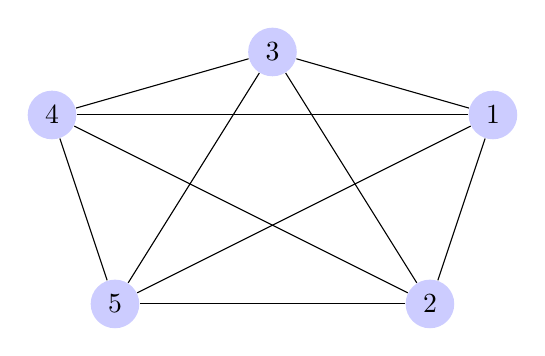
\begin{tikzpicture}
  [scale=.8,auto=left,every node/.style={circle,fill=blue!20} ]%edge/.style={bend left}]
  \node (n4) at (4,8)  {4};
  \node (n3) at (7.5,9)  {3};
  \node (n1) at (11,8) {1};
  \node (n2) at (10,5)  {2};
  \node (n5) at (5,5)  {5};`

  \foreach \from/\to in {n1/n2,n1/n3,n1/n4,n1/n5,n2/n3,n2/n4,n2/n5,n3/n4,n3/n5,n4/n5}
    \draw (\from) -- (\to);

\end{tikzpicture}


Here, every node is connected to every one of the rest. Therefore, every node is identical to every one else. In this case, 
every assignment of numbers $1\ldots n$ to the nodes yields the same graph. Therefore to solve this instance, we consider a random labeling of our nodes, and we compute the cuts at all integer points between 1 and n. 


Another instance, could be this graph.

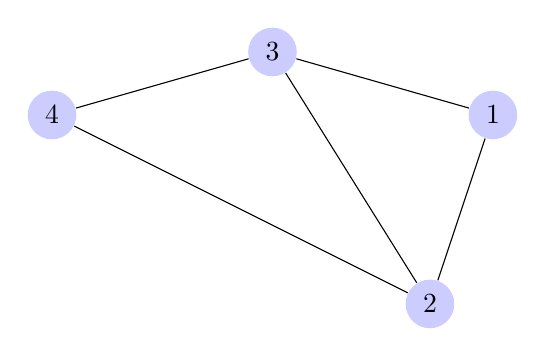
\begin{tikzpicture}
  [scale=.8,auto=left,every node/.style={circle,fill=blue!20} ]%edge/.style={bend left}]
  \node (n4) at (4,8)  {4};
  \node (n3) at (7.5,9)  {3};
  \node (n1) at (11,8) {1};
  \node (n2) at (10,5)  {2};

  \tikzset{EdgeStyle/.append style = {bend left}}
  \foreach \from/\to in {n1/n2,n1/n3,n2/n3,n2/n4,n3/n4}
    \draw (\from) -> (\to);

\end{tikzpicture}


Here, the assignment matters, and one possible solution could be: f(1)=1, f(2)=2, f(3)=4, f(4)=3. This was found using exhaustive search. However, in order to attack the problem in a more intuitive manner, it would be more suitable to have visualize the problem as follows: Given graph G, create a drawing of G such that the nodes are placed on a straight horizontal line.
The objective is to minimize the maximum number of edges that exist in the space between two consecutive nodes. 

\textbf{TODO: FIX GRAPH BELOW}



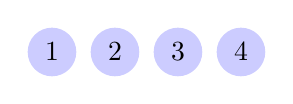
\begin{tikzpicture}
  [scale=.8,auto=left,every node/.style={circle,fill=blue!20} ]%edge/.style={bend left}]
  \node (n4) at (4,1)  {4};
  \node (n3) at (3,1)  {3};
  \node (n1) at (1,1) {1};
  \node (n2) at (2,1)  {2};

  \foreach \from/\to in {n1/n2,n1/n3,n2/n3,n2/n4,n3/n4}
    \draw (\from) (\to);
\end{tikzpicture}




